\documentclass[12pt]{article}\usepackage[]{graphicx}\usepackage[]{color}
%% maxwidth is the original width if it is less than linewidth
%% otherwise use linewidth (to make sure the graphics do not exceed the margin)
\makeatletter
\def\maxwidth{ %
  \ifdim\Gin@nat@width>\linewidth
    \linewidth
  \else
    \Gin@nat@width
  \fi
}
\makeatother

\definecolor{fgcolor}{rgb}{0.345, 0.345, 0.345}
\newcommand{\hlnum}[1]{\textcolor[rgb]{0.686,0.059,0.569}{#1}}%
\newcommand{\hlstr}[1]{\textcolor[rgb]{0.192,0.494,0.8}{#1}}%
\newcommand{\hlcom}[1]{\textcolor[rgb]{0.678,0.584,0.686}{\textit{#1}}}%
\newcommand{\hlopt}[1]{\textcolor[rgb]{0,0,0}{#1}}%
\newcommand{\hlstd}[1]{\textcolor[rgb]{0.345,0.345,0.345}{#1}}%
\newcommand{\hlkwa}[1]{\textcolor[rgb]{0.161,0.373,0.58}{\textbf{#1}}}%
\newcommand{\hlkwb}[1]{\textcolor[rgb]{0.69,0.353,0.396}{#1}}%
\newcommand{\hlkwc}[1]{\textcolor[rgb]{0.333,0.667,0.333}{#1}}%
\newcommand{\hlkwd}[1]{\textcolor[rgb]{0.737,0.353,0.396}{\textbf{#1}}}%
\let\hlipl\hlkwb

\usepackage{framed}
\makeatletter
\newenvironment{kframe}{%
 \def\at@end@of@kframe{}%
 \ifinner\ifhmode%
  \def\at@end@of@kframe{\end{minipage}}%
  \begin{minipage}{\columnwidth}%
 \fi\fi%
 \def\FrameCommand##1{\hskip\@totalleftmargin \hskip-\fboxsep
 \colorbox{shadecolor}{##1}\hskip-\fboxsep
     % There is no \\@totalrightmargin, so:
     \hskip-\linewidth \hskip-\@totalleftmargin \hskip\columnwidth}%
 \MakeFramed {\advance\hsize-\width
   \@totalleftmargin\z@ \linewidth\hsize
   \@setminipage}}%
 {\par\unskip\endMakeFramed%
 \at@end@of@kframe}
\makeatother

\definecolor{shadecolor}{rgb}{.97, .97, .97}
\definecolor{messagecolor}{rgb}{0, 0, 0}
\definecolor{warningcolor}{rgb}{1, 0, 1}
\definecolor{errorcolor}{rgb}{1, 0, 0}
\newenvironment{knitrout}{}{} % an empty environment to be redefined in TeX

\usepackage{alltt}
 
\usepackage[margin=1in]{geometry}
\usepackage{amsmath,amsthm,amssymb, mathtools}
\usepackage[T1]{fontenc}
\usepackage{lmodern}
\usepackage{fixltx2e}
\usepackage[shortlabels]{enumitem}
 
\newcommand{\N}{\mathbb{N}}
\newcommand{\R}{\mathbb{R}}
\newcommand{\Z}{\mathbb{Z}}
\newcommand{\Q}{\mathbb{Q}}

\newenvironment{theorem}[2][Theorem]{\begin{trivlist}
\item[\hskip \labelsep {\bfseries #1}\hskip \labelsep {\bfseries #2.}]}{\end{trivlist}}
\newenvironment{lemma}[2][Lemma]{\begin{trivlist}
\item[\hskip \labelsep {\bfseries #1}\hskip \labelsep {\bfseries #2.}]}{\end{trivlist}}
\newenvironment{exercise}[2][Exercise]{\begin{trivlist}
\item[\hskip \labelsep {\bfseries #1}\hskip \labelsep {\bfseries #2.}]}{\end{trivlist}}
\newenvironment{problem}[2][Problem]{\begin{trivlist}
\item[\hskip \labelsep {\bfseries #1}\hskip \labelsep {\bfseries #2.}]}{\end{trivlist}}
\newenvironment{question}[2][Question]{\begin{trivlist}
\item[\hskip \labelsep {\bfseries #1}\hskip \labelsep {\bfseries #2.}]}{\end{trivlist}}
\newenvironment{corollary}[2][Corollary]{\begin{trivlist}
\item[\hskip \labelsep {\bfseries #1}\hskip \labelsep {\bfseries #2.}]}{\end{trivlist}}
\newcommand{\textfrac}[2]{\dfrac{\text{#1}}{\text{#2}}}
\IfFileExists{upquote.sty}{\usepackage{upquote}}{}
\begin{document}

\title{Statistical Rethinking: Chapter 5 - Multivariate Linear Models}

\author{Chris Hayduk}
\date{\today}

\maketitle




\section{Easy}

\begin{problem}{5E1}
\text{ }\\
Which of the linear models below are multiple linear regressions?
\begin{enumerate}
	\item $\mu$\textsubscript{i} = $\alpha$ + $\beta$x\textsubscript{i}
	\item $\mu$\textsubscript{i} = $\beta$\textsubscript{x}x\textsubscript{i} + $\beta$\textsubscript{z}z\textsubscript{i}
	\item $\mu$\textsubscript{i} = $\alpha$ + $\beta$(x\textsubscript{i} - z\textsubscript{i})
	\item $\mu$\textsubscript{i} = $\alpha$ + $\beta$\textsubscript{x}x\textsubscript{i} + $\beta$\textsubscript{z}z\textsubscript{i}
\end{enumerate}
\end{problem}

Linear models 2 and 4 are multiple linear regressions.

\begin{problem}{5E2}
\text{ }\\
Write down a multiple regression to evaluate the claim: \textit{Animal diversity is linearly related to latitude, but only after controlling for plant diversity.} You just need to write down the model definition.
\end{problem}

\begin{center}
animal diversity\textsubscript{i} $\sim$ Normal($\mu$\textsubscript{i}, $\sigma$)\\
$\mu$\textsubscript{i} = $\beta$\textsubscript{latitude}latitude\textsubscript{i} + $\beta$\textsubscript{diversity}diversity\textsubscript{i}\\
$\beta$\textsubscript{latitude} $\sim$ Normal(0, 10)\\
$\beta$\textsubscript{diversity} $\sim$ Normal(0, 10)\\
$\sigma$ $\sim$ Uniform(0, 10)
\end{center}

\begin{problem}{5E3}
\text{ }\\
Write down a multiple regression to evaluate the claim: \textit{Neither amount of funding nor size of laboratory is by itself a good predictor of time to PhD degree; but together these variables are both positively associated with time to degree.} Write down the model definition and indicate which side of zero each slope parameter should be on.
\end{problem}

\begin{center}
time\textsubscript{i} $\sim$ Normal($\mu$\textsubscript{i}, $\sigma$)\\
$\mu$\textsubscript{i} = $\beta$\textsubscript{lab size}lab size\textsubscript{i} + $\beta$\textsubscript{funding}funding\textsubscript{i}\\
$\beta$\textsubscript{lab size} $\sim$ Normal(0, 10)\\
$\beta$\textsubscript{funding} $\sim$ Normal(0, 10)\\
$\sigma$ $\sim$ Uniform(0, 10)
\end{center}

Both parameters should have slopes greater than zero since the problem specifies that "together the variables are both positively associated with time to degree".

\begin{problem}{5E4}
\text{ }\\
Suppose you have a single categorical predictor with 4 levels (unique values), labeled A, B, C, and D. Let A\textsubscript{i} be an indicator variable that is 1 where case \textit{i} is in category A. Also suppose B\textsubscript{i}, C\textsubscript{i}, and D\textsubscript{i} for the other categories. Now which of the following linear models are inferentially equivalent ways to include the categorical variable in a regression? Models are inferentially equivalent when it's possible to compute one posterior distribution from the posterior distribution of another model.
\begin{enumerate}
	\item $\mu$\textsubscript{i} = $\alpha$ + $\beta$\textsubscript{A}A\textsubscript{i} + $\beta$\textsubscript{B}B\textsubscript{i} + $\beta$\textsubscript{D}D\textsubscript{i}
	\item $\mu$\textsubscript{i} = $\alpha$ + $\beta$\textsubscript{A}A\textsubscript{i} + $\beta$\textsubscript{B}B\textsubscript{i} + $\beta$\textsubscript{C}C\textsubscript{i} + $\beta$\textsubscript{D}D\textsubscript{i}
	\item $\mu$\textsubscript{i} = $\alpha$ + $\beta$\textsubscript{B}B\textsubscript{i} + $\beta$\textsubscript{C}C\textsubscript{i} + $\beta$\textsubscript{D}D\textsubscript{i}
	\item $\mu$\textsubscript{i} = $\alpha$\textsubscript{A}A\textsubscript{i} + $\alpha$\textsubscript{B}B\textsubscript{i} + $\alpha$\textsubscript{C}C\textsubscript{i} + $\alpha$\textsubscript{D}D\textsubscript{i}
	\item $\mu$\textsubscript{i} = $\alpha$\textsubscript{i}(1 - B\textsubscript{i} - C\textsubscript{i} - D\textsubscript{i}) + $\alpha$\textsubscript{B}B\textsubscript{i} + $\alpha$\textsubscript{C}C\textsubscript{i} + $\alpha$\textsubscript{D}D\textsubscript{i}
\end{enumerate}
\end{problem}

Models 1, 3, 4, and 5 are all inferentially equivalent.

\section{Medium}

\begin{problem}{5M1}
\text{ }\\
Invent your own example of a spurious correlation. An outcome variable should be correlated with both predictor variables. But when both predictors are entered in the same model, the correlation between the outcome and one of the predictors should mostly vanish (or at least be greatly reduced).
\end{problem}

\begin{knitrout}
\definecolor{shadecolor}{rgb}{0.969, 0.969, 0.969}\color{fgcolor}\begin{kframe}
\begin{alltt}
\hlstd{N} \hlkwb{<-} \hlnum{1e4}
\hlstd{x.real} \hlkwb{<-} \hlkwd{rnorm}\hlstd{(}\hlkwc{n} \hlstd{= N,} \hlkwc{mean} \hlstd{=} \hlnum{1}\hlstd{,} \hlkwc{sd} \hlstd{=} \hlnum{1}\hlstd{)}
\hlstd{x.spurious} \hlkwb{<-} \hlkwd{rnorm}\hlstd{(}\hlkwc{n} \hlstd{= N,} \hlkwc{mean} \hlstd{= x.real)}
\hlstd{y} \hlkwb{<-} \hlkwd{rnorm}\hlstd{(}\hlkwc{n} \hlstd{= N,} \hlkwc{mean} \hlstd{= x.real)}

\hlstd{df} \hlkwb{<-} \hlkwd{data.frame}\hlstd{(}\hlkwc{y} \hlstd{= y,} \hlkwc{x.real} \hlstd{= x.real,} \hlkwc{x.spurious} \hlstd{= x.spurious)}
\hlkwd{pairs}\hlstd{(df)}
\end{alltt}
\end{kframe}
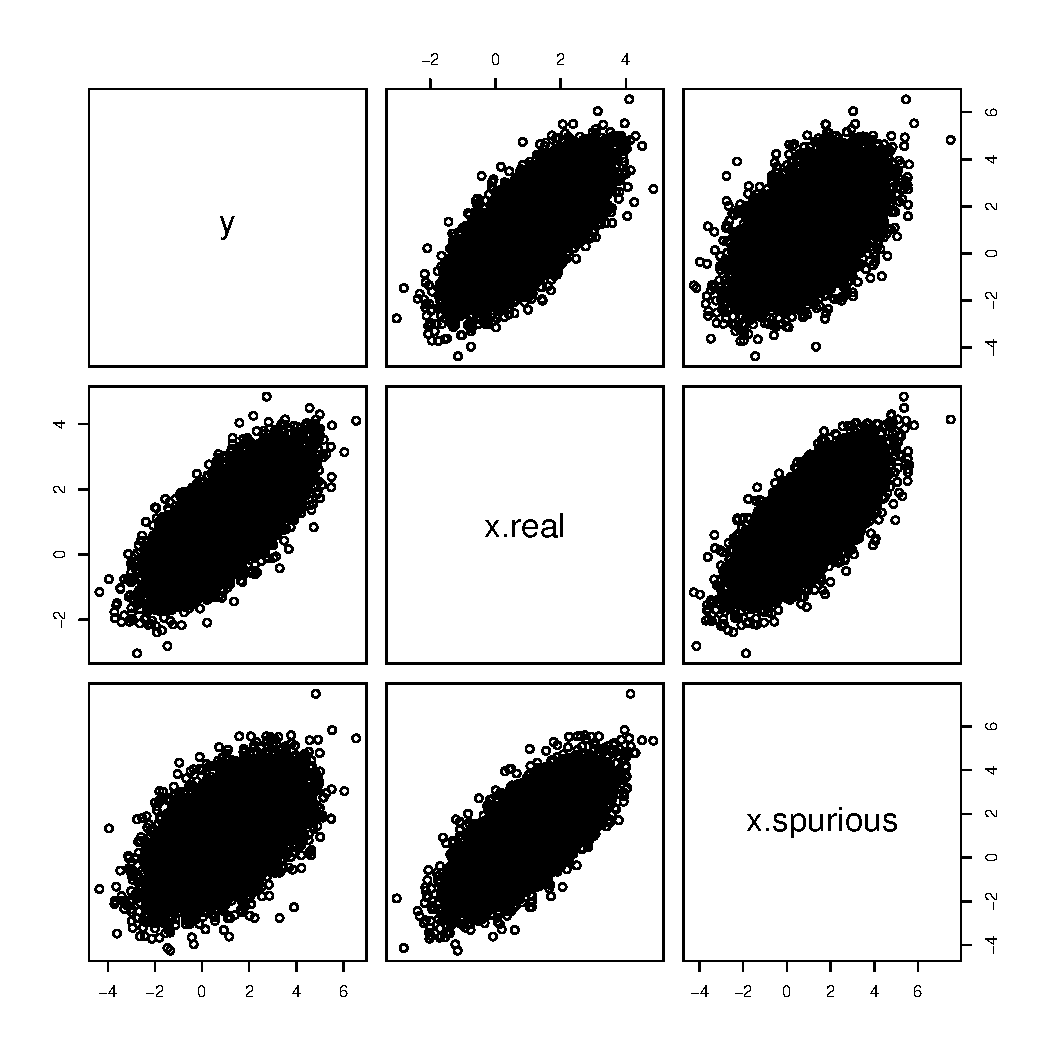
\includegraphics[width=\maxwidth]{figure/unnamed-chunk-2-1} 
\begin{kframe}\begin{alltt}
\hlstd{model} \hlkwb{<-} \hlkwd{lm}\hlstd{(y} \hlopt{~} \hlstd{x.real} \hlopt{+} \hlstd{x.spurious)}
\hlkwd{precis}\hlstd{(model)}
\end{alltt}
\begin{verbatim}
##             Mean StdDev  5.5% 94.5%
## (Intercept) 0.01   0.01 -0.01  0.03
## x.real      1.00   0.01  0.97  1.02
## x.spurious  0.00   0.01 -0.02  0.01
\end{verbatim}
\end{kframe}
\end{knitrout}

\begin{problem}{5M2}
\text{ }\\
Invent your own example of a masked relationship. An outcome variable should be correlated with both predictor variables, but in opposite directions. And the two predictor variables should be correlated with one another.
\end{problem}

\begin{knitrout}
\definecolor{shadecolor}{rgb}{0.969, 0.969, 0.969}\color{fgcolor}\begin{kframe}
\begin{alltt}
\hlstd{N} \hlkwb{<-} \hlnum{1e4}
\hlstd{rho} \hlkwb{<-} \hlnum{0.7}

\hlstd{x.pos} \hlkwb{<-} \hlkwd{rnorm}\hlstd{(N)}
\hlstd{x.neg} \hlkwb{<-} \hlkwd{rnorm}\hlstd{(N, rho}\hlopt{*}\hlstd{x.pos,} \hlkwd{sqrt}\hlstd{(}\hlnum{1}\hlopt{-}\hlstd{rho}\hlopt{^}\hlnum{2}\hlstd{))}
\hlstd{y} \hlkwb{<-} \hlkwd{rnorm}\hlstd{(N, x.pos} \hlopt{-} \hlstd{x.neg)}

\hlstd{df} \hlkwb{<-} \hlkwd{data.frame}\hlstd{(}\hlkwc{y} \hlstd{= y,} \hlkwc{x.pos} \hlstd{= x.pos,} \hlkwc{x.neg} \hlstd{= x.neg)}
\hlkwd{pairs}\hlstd{(df)}
\end{alltt}
\end{kframe}
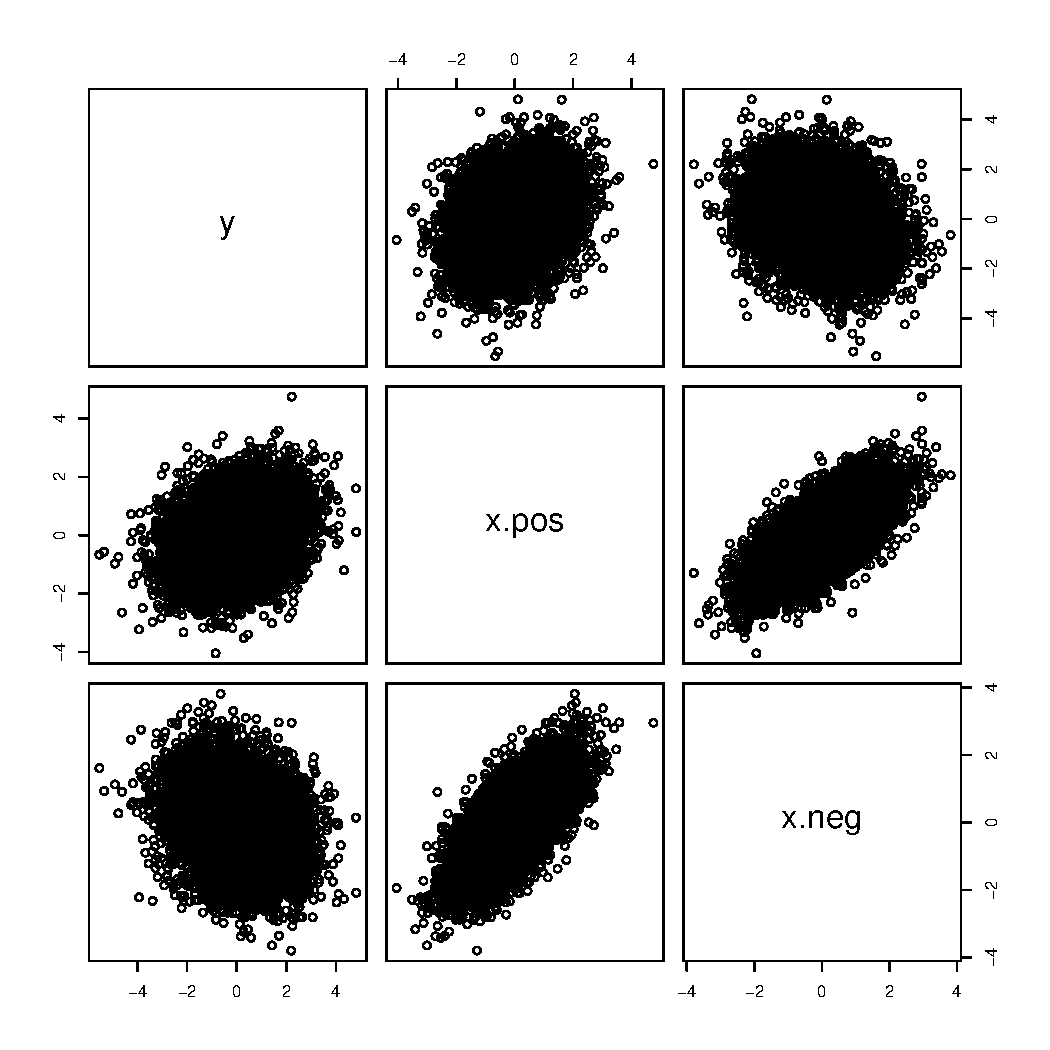
\includegraphics[width=\maxwidth]{figure/unnamed-chunk-3-1} 
\begin{kframe}\begin{alltt}
\hlstd{model} \hlkwb{<-} \hlkwd{lm}\hlstd{(y} \hlopt{~} \hlstd{x.pos} \hlopt{+} \hlstd{x.neg)}
\hlkwd{precis}\hlstd{(model)}
\end{alltt}
\begin{verbatim}
##              Mean StdDev  5.5% 94.5%
## (Intercept)  0.01   0.01 -0.01  0.02
## x.pos        1.00   0.01  0.97  1.02
## x.neg       -0.99   0.01 -1.01 -0.97
\end{verbatim}
\end{kframe}
\end{knitrout}

\begin{problem}{5M3}
\text{ }\\
It is sometimes observed that the best predictor of fire risk is the presence of firefighters - States and localities with many firefighters also have more fires. Presumably firefightes do not \textit{cause} fires. Nevertheless, this is not a spurious correlation. Instead fires cause firefighters. Consider the same reversal of causal inference in the context of the divorice and marriage data. How might a high divorce rate cause a higher marriage rate? Can you think of a way to evaluate this relationship, using multiple regression?
\end{problem}

A high divorce rate may cause a higher marriage rate because people who are divorced may get married multiple times throughout their lives.

\begin{problem}{5M4}
\text{ }\\
In the divorce data, States with high numbers of Mormons have much lower divorce rates than the regression models expected. Find a list of LDS population by State and use those numbers as a predictor variable, predicting divorce rate using marriage rate, median age at marriage, and percent LDS population (possibly standardized). You may want to consider transformations of the raw percent LDS variable.
\end{problem}

\begin{knitrout}
\definecolor{shadecolor}{rgb}{0.969, 0.969, 0.969}\color{fgcolor}\begin{kframe}
\begin{alltt}
\hlkwd{setwd}\hlstd{(}\hlkwd{dirname}\hlstd{(rstudioapi}\hlopt{::}\hlkwd{getActiveDocumentContext}\hlstd{()}\hlopt{$}\hlstd{path))}
\end{alltt}


{\ttfamily\noindent\bfseries\color{errorcolor}{\#\# Error: RStudio not running}}\begin{alltt}
\hlstd{mormon} \hlkwb{<-} \hlkwd{read_excel}\hlstd{(}\hlstr{"Mormon.xlsx"}\hlstd{)}

\hlkwd{data}\hlstd{(WaffleDivorce)}

\hlstd{d} \hlkwb{<-} \hlstd{WaffleDivorce}

\hlkwd{names}\hlstd{(mormon)} \hlkwb{<-} \hlkwd{c}\hlstd{(}\hlstr{"Location"}\hlstd{,} \hlstr{"MormonPop"}\hlstd{,} \hlstr{"StatePop"}\hlstd{,} \hlstr{"PercMormon"}\hlstd{)}

\hlstd{mormon} \hlkwb{<-} \hlstd{mormon[,}\hlkwd{c}\hlstd{(}\hlstr{"Location"}\hlstd{,} \hlstr{"MormonPop"}\hlstd{,} \hlstr{"PercMormon"}\hlstd{)]}

\hlstd{d} \hlkwb{<-} \hlkwd{left_join}\hlstd{(d, mormon)}

\hlstd{d}\hlopt{$}\hlstd{MedianAgeMarriage.s} \hlkwb{<-} \hlstd{(d}\hlopt{$}\hlstd{MedianAgeMarriage} \hlopt{-} \hlkwd{mean}\hlstd{(d}\hlopt{$}\hlstd{MedianAgeMarriage))}\hlopt{/}\hlkwd{sd}\hlstd{(d}\hlopt{$}\hlstd{MedianAgeMarriage)}

\hlstd{d}\hlopt{$}\hlstd{Marriage.s} \hlkwb{<-} \hlstd{(d}\hlopt{$}\hlstd{Marriage} \hlopt{-} \hlkwd{mean}\hlstd{(d}\hlopt{$}\hlstd{Marriage))}\hlopt{/}\hlkwd{sd}\hlstd{(d}\hlopt{$}\hlstd{Marriage)}

\hlstd{d}\hlopt{$}\hlstd{PercMormon.s} \hlkwb{<-} \hlstd{(d}\hlopt{$}\hlstd{PercMormon} \hlopt{-} \hlkwd{mean}\hlstd{(d}\hlopt{$}\hlstd{PercMormon))}\hlopt{/}\hlkwd{sd}\hlstd{(d}\hlopt{$}\hlstd{PercMormon)}

\hlstd{model} \hlkwb{<-} \hlkwd{map}\hlstd{(}
  \hlkwd{alist}\hlstd{(}
    \hlstd{Divorce} \hlopt{~} \hlkwd{dnorm}\hlstd{(mu, sigma),}
    \hlstd{mu} \hlkwb{<-} \hlstd{a} \hlopt{+} \hlstd{b1} \hlopt{*} \hlstd{Marriage.s} \hlopt{+ +} \hlstd{b2} \hlopt{*} \hlstd{MedianAgeMarriage.s} \hlopt{+} \hlstd{b3} \hlopt{*} \hlstd{PercMormon.s,}
    \hlstd{a} \hlopt{~} \hlkwd{dnorm}\hlstd{(}\hlnum{10}\hlstd{,} \hlnum{10}\hlstd{),}
    \hlstd{b1} \hlopt{~} \hlkwd{dnorm}\hlstd{(}\hlnum{0}\hlstd{,} \hlnum{1}\hlstd{),}
    \hlstd{b2} \hlopt{~} \hlkwd{dnorm}\hlstd{(}\hlnum{0}\hlstd{,} \hlnum{1}\hlstd{),}
    \hlstd{b3} \hlopt{~} \hlkwd{dnorm}\hlstd{(}\hlnum{0}\hlstd{,} \hlnum{1}\hlstd{),}
    \hlstd{sigma} \hlopt{~} \hlkwd{dunif}\hlstd{(}\hlnum{0}\hlstd{,} \hlnum{10}\hlstd{)}
  \hlstd{),} \hlkwc{data} \hlstd{= d)}

\hlkwd{precis}\hlstd{(model)}
\end{alltt}
\begin{verbatim}
##        Mean StdDev  5.5% 94.5%
## a      9.69   0.19  9.38  9.99
## b1     0.06   0.27 -0.38  0.49
## b2    -1.27   0.27 -1.70 -0.85
## b3    -0.58   0.22 -0.93 -0.23
## sigma  1.34   0.13  1.13  1.56
\end{verbatim}
\begin{alltt}
\hlkwd{plot}\hlstd{(}\hlkwd{precis}\hlstd{(model))}
\end{alltt}
\end{kframe}
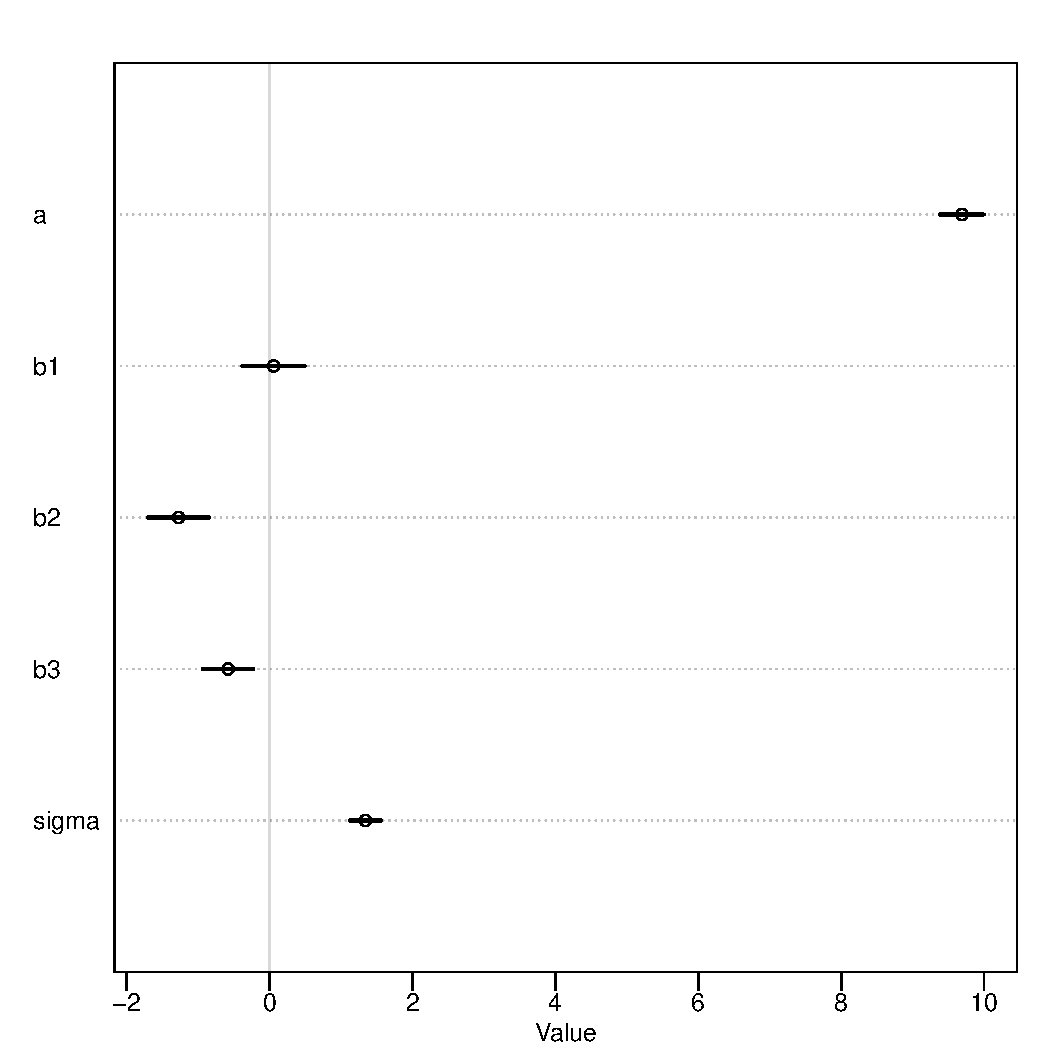
\includegraphics[width=\maxwidth]{figure/unnamed-chunk-4-1} 

\end{knitrout}

\begin{problem}{5M5}
\text{ }\\
One way to reason through multiple causation hypotheses is to imagine detailed mechanisms through which predictor variables may influence outcomes. For example, it is sometimes argued that the price of gasoline (predictor variable) is positiviely associated with lower obesity rates (outcome variable). However, there are at least two important mechanisms by which the price of gas could reduce obesity. First, it could lead to less driving and therefore more exercise. Second, it could lead to less driving, which leads to less eating out, which leads to less consumption of huge restaurant meals. Can you outline one or more multiple regressions that address these two mechanisms? Assume you can have any predictor data you need.
\end{problem}

Model 1:
\begin{center}
obesity rate\textsubscript{i} $\sim$ Normal($\mu$\textsubscript{i}, $\sigma$)\\
$\mu$\textsubscript{i} = $\beta$\textsubscript{gas}gas price\textsubscript{i} + $\beta$\textsubscript{driving}hours driving per year per capita\textsubscript{i}\\
$\beta$\textsubscript{gas} $\sim$ Normal(0, 10)\\
$\beta$\textsubscript{driving} $\sim$ Normal(0, 10)\\
$\sigma$ $\sim$ Uniform(0, 10)
\end{center}

Model 2:
\begin{center}
obesity rate\textsubscript{i} $\sim$ Normal($\mu$\textsubscript{i}, $\sigma$)\\
$\mu$\textsubscript{i} = $\beta$\textsubscript{gas}gas price\textsubscript{i} + $\beta$\textsubscript{restaurant}restaurant trips per year per capita\textsubscript{i}\\
$\beta$\textsubscript{gas} $\sim$ Normal(0, 10)\\
$\beta$\textsubscript{restaurant} $\sim$ Normal(0, 10)\\
$\sigma$ $\sim$ Uniform(0, 10)
\end{center}

\section{Hard}

All three exercises below use the same data, data(foxes) (part of rethinking). The urban fox (\textit{Vulpes vulpes}) is a successful exploiter of human habitat. Since urbran foxes move in packs and defend territories, data on haitat quality and population density is also included. The data frame has fix columns:
\begin{enumerate}
	\item group: Number of the social group the individual fox belongs to
	\item avgfood: The average amount of food available in the territory
	\item groupsize: The number of foxes in the social group
	\item area: Size of the territory
	\item weight: Body weight of the individual fox
\end{enumerate}

\begin{problem}{5H1}
\text{ }\\
Fit two bivariate Gaussian regressions, using map: (1) body weight as a linear function of territory size (area), and (2) body weight as a linear function of groupsize. Plot the results of these regressions, displaying the MAP regression line and 95\% interval of the mean. Is either variable important for predicting fox body weight?
\end{problem}

\begin{knitrout}
\definecolor{shadecolor}{rgb}{0.969, 0.969, 0.969}\color{fgcolor}\begin{kframe}
\begin{alltt}
\hlkwd{data}\hlstd{(foxes)}

\hlstd{d} \hlkwb{<-} \hlstd{foxes}

\hlstd{model1} \hlkwb{<-} \hlkwd{map}\hlstd{(}
  \hlkwd{alist}\hlstd{(}
    \hlstd{weight} \hlopt{~} \hlkwd{dnorm}\hlstd{(mu, sigma),}
    \hlstd{mu} \hlkwb{<-} \hlstd{a} \hlopt{+} \hlstd{b} \hlopt{*} \hlstd{area,}
    \hlstd{a} \hlopt{~} \hlkwd{dnorm}\hlstd{(}\hlnum{10}\hlstd{,} \hlnum{10}\hlstd{),}
    \hlstd{b} \hlopt{~} \hlkwd{dnorm}\hlstd{(}\hlnum{0}\hlstd{,} \hlnum{100}\hlstd{),}
    \hlstd{sigma} \hlopt{~} \hlkwd{dunif}\hlstd{(}\hlnum{0}\hlstd{,} \hlnum{10}\hlstd{)}
  \hlstd{),} \hlkwc{data} \hlstd{= d)}

\hlstd{model2} \hlkwb{<-} \hlkwd{map}\hlstd{(}
  \hlkwd{alist}\hlstd{(}
    \hlstd{weight} \hlopt{~} \hlkwd{dnorm}\hlstd{(mu, sigma),}
    \hlstd{mu} \hlkwb{<-} \hlstd{a} \hlopt{+} \hlstd{b} \hlopt{*} \hlstd{groupsize,}
    \hlstd{a} \hlopt{~} \hlkwd{dnorm}\hlstd{(}\hlnum{10}\hlstd{,} \hlnum{10}\hlstd{),}
    \hlstd{b} \hlopt{~} \hlkwd{dnorm}\hlstd{(}\hlnum{0}\hlstd{,} \hlnum{100}\hlstd{),}
    \hlstd{sigma} \hlopt{~} \hlkwd{dunif}\hlstd{(}\hlnum{0}\hlstd{,} \hlnum{10}\hlstd{)}
  \hlstd{),} \hlkwc{data} \hlstd{= d)}

\hlstd{area.seq} \hlkwb{<-} \hlkwd{seq}\hlstd{(}\hlkwc{from} \hlstd{=} \hlkwd{round}\hlstd{(}\hlkwd{min}\hlstd{(d}\hlopt{$}\hlstd{area),} \hlnum{1}\hlstd{),} \hlkwc{to} \hlstd{=} \hlkwd{round}\hlstd{(}\hlkwd{max}\hlstd{(d}\hlopt{$}\hlstd{area),}\hlnum{1}\hlstd{),} \hlkwc{length.out} \hlstd{=} \hlnum{100}\hlstd{)}

\hlstd{groupsize.seq} \hlkwb{<-} \hlkwd{seq}\hlstd{(}\hlkwc{from} \hlstd{=} \hlkwd{round}\hlstd{(}\hlkwd{min}\hlstd{(d}\hlopt{$}\hlstd{groupsize),} \hlnum{1}\hlstd{),} \hlkwc{to} \hlstd{=} \hlkwd{round}\hlstd{(}\hlkwd{max}\hlstd{(d}\hlopt{$}\hlstd{groupsize),}\hlnum{1}\hlstd{),} \hlkwc{length.out} \hlstd{=} \hlnum{100}\hlstd{)}

\hlstd{mu1} \hlkwb{<-} \hlkwd{link}\hlstd{(model1,} \hlkwc{data} \hlstd{=} \hlkwd{data.frame}\hlstd{(}\hlkwc{area}\hlstd{=area.seq))}
\end{alltt}
\begin{verbatim}
## [ 100 / 1000 ]
[ 200 / 1000 ]
[ 300 / 1000 ]
[ 400 / 1000 ]
[ 500 / 1000 ]
[ 600 / 1000 ]
[ 700 / 1000 ]
[ 800 / 1000 ]
[ 900 / 1000 ]
[ 1000 / 1000 ]

\end{verbatim}
\begin{alltt}
\hlstd{mu1.PI} \hlkwb{<-} \hlkwd{apply}\hlstd{(mu1,} \hlnum{2}\hlstd{, PI,} \hlnum{0.95}\hlstd{)}

\hlstd{mu2} \hlkwb{<-} \hlkwd{link}\hlstd{(model2,} \hlkwc{data} \hlstd{=} \hlkwd{data.frame}\hlstd{(}\hlkwc{groupsize} \hlstd{= groupsize.seq))}
\end{alltt}
\begin{verbatim}
## [ 100 / 1000 ]
[ 200 / 1000 ]
[ 300 / 1000 ]
[ 400 / 1000 ]
[ 500 / 1000 ]
[ 600 / 1000 ]
[ 700 / 1000 ]
[ 800 / 1000 ]
[ 900 / 1000 ]
[ 1000 / 1000 ]

\end{verbatim}
\begin{alltt}
\hlstd{mu2.PI} \hlkwb{<-} \hlkwd{apply}\hlstd{(mu2,} \hlnum{2}\hlstd{, PI,} \hlnum{0.95}\hlstd{)}

\hlkwd{par}\hlstd{(}\hlkwc{mfrow}\hlstd{=}\hlkwd{c}\hlstd{(}\hlnum{1}\hlstd{,}\hlnum{2}\hlstd{))}

\hlkwd{plot}\hlstd{(weight} \hlopt{~} \hlstd{area,} \hlkwc{data} \hlstd{= d,} \hlkwc{col}\hlstd{=rangi2)}
\hlkwd{abline}\hlstd{(model1)}
\hlkwd{shade}\hlstd{(mu1.PI, area.seq)}

\hlkwd{plot}\hlstd{(weight} \hlopt{~} \hlstd{groupsize,} \hlkwc{data} \hlstd{= d,} \hlkwc{col} \hlstd{= rangi2)}
\hlkwd{abline}\hlstd{(model2)}
\hlkwd{shade}\hlstd{(mu2.PI, groupsize.seq)}
\end{alltt}
\end{kframe}
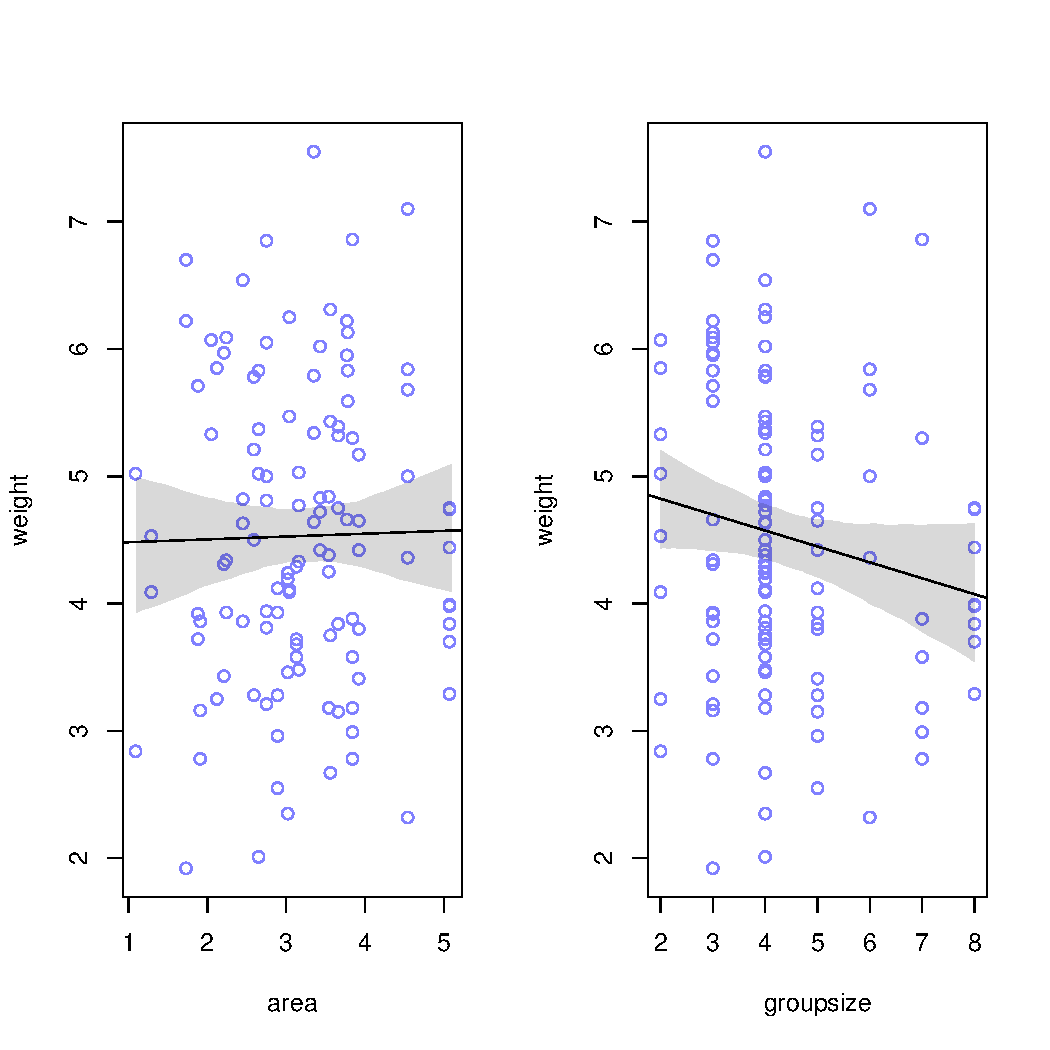
\includegraphics[width=\maxwidth]{figure/unnamed-chunk-5-1} 

\end{knitrout}

Neither predictor appears to be heavily associated with weight, although group size does slightly better than area.

\begin{problem}{5H2}
\text{ }\\
Now fit a multiple linear regression with weight as the outcome and both area and groupsize as predictor variables. Plot the predictions of the model for each predictor, holding the other predictor constant at its mean. What does this model say about the importance of each variable? Why do you get different results than you got in the exercise above?
\end{problem}

\begin{knitrout}
\definecolor{shadecolor}{rgb}{0.969, 0.969, 0.969}\color{fgcolor}\begin{kframe}
\begin{alltt}
\hlstd{model3} \hlkwb{<-} \hlkwd{map}\hlstd{(}
  \hlkwd{alist}\hlstd{(}
    \hlstd{weight} \hlopt{~} \hlkwd{dnorm}\hlstd{(mu, sigma),}
    \hlstd{mu} \hlkwb{<-} \hlstd{a} \hlopt{+} \hlstd{b1} \hlopt{*} \hlstd{area} \hlopt{+} \hlstd{b2} \hlopt{*} \hlstd{groupsize,}
    \hlstd{a} \hlopt{~} \hlkwd{dnorm}\hlstd{(}\hlnum{10}\hlstd{,} \hlnum{10}\hlstd{),}
    \hlstd{b1} \hlopt{~} \hlkwd{dnorm}\hlstd{(}\hlnum{0}\hlstd{,} \hlnum{100}\hlstd{),}
    \hlstd{b2} \hlopt{~} \hlkwd{dnorm}\hlstd{(}\hlnum{0}\hlstd{,} \hlnum{100}\hlstd{),}
    \hlstd{sigma} \hlopt{~} \hlkwd{dunif}\hlstd{(}\hlnum{0}\hlstd{,} \hlnum{10}\hlstd{)}
  \hlstd{),} \hlkwc{data} \hlstd{= d)}

\hlkwd{precis}\hlstd{(model3)}
\end{alltt}
\begin{verbatim}
##        Mean StdDev  5.5% 94.5%
## a      4.46   0.37  3.87  5.05
## b1     0.62   0.20  0.30  0.94
## b2    -0.43   0.12 -0.63 -0.24
## sigma  1.12   0.07  1.00  1.24
\end{verbatim}
\begin{alltt}
\hlstd{A.avg} \hlkwb{<-} \hlkwd{mean}\hlstd{(d}\hlopt{$}\hlstd{area)}
\hlstd{G.avg} \hlkwb{<-} \hlkwd{mean}\hlstd{(d}\hlopt{$}\hlstd{groupsize)}

\hlstd{pred.data1} \hlkwb{<-}\hlkwd{data.frame}\hlstd{(}\hlkwc{area} \hlstd{= area.seq,} \hlkwc{groupsize} \hlstd{= G.avg)}
\hlstd{pred.data2} \hlkwb{<-} \hlkwd{data.frame}\hlstd{(}\hlkwc{area} \hlstd{= A.avg,} \hlkwc{groupsize} \hlstd{= groupsize.seq)}

\hlstd{mu1} \hlkwb{<-} \hlkwd{link}\hlstd{(model3,} \hlkwc{data} \hlstd{= pred.data1)}
\end{alltt}
\begin{verbatim}
## [ 100 / 1000 ]
[ 200 / 1000 ]
[ 300 / 1000 ]
[ 400 / 1000 ]
[ 500 / 1000 ]
[ 600 / 1000 ]
[ 700 / 1000 ]
[ 800 / 1000 ]
[ 900 / 1000 ]
[ 1000 / 1000 ]

\end{verbatim}
\begin{alltt}
\hlstd{mu1.mean} \hlkwb{<-} \hlkwd{apply}\hlstd{(mu1,} \hlnum{2}\hlstd{, mean)}
\hlstd{mu1.PI} \hlkwb{<-} \hlkwd{apply}\hlstd{(mu1,} \hlnum{2}\hlstd{, PI,} \hlnum{0.95}\hlstd{)}

\hlstd{mu2} \hlkwb{<-} \hlkwd{link}\hlstd{(model3,} \hlkwc{data} \hlstd{= pred.data2)}
\end{alltt}
\begin{verbatim}
## [ 100 / 1000 ]
[ 200 / 1000 ]
[ 300 / 1000 ]
[ 400 / 1000 ]
[ 500 / 1000 ]
[ 600 / 1000 ]
[ 700 / 1000 ]
[ 800 / 1000 ]
[ 900 / 1000 ]
[ 1000 / 1000 ]

\end{verbatim}
\begin{alltt}
\hlstd{mu2.mean} \hlkwb{<-} \hlkwd{apply}\hlstd{(mu2,} \hlnum{2}\hlstd{, mean)}
\hlstd{mu2.PI} \hlkwb{<-} \hlkwd{apply}\hlstd{(mu2,} \hlnum{2}\hlstd{, PI,} \hlnum{0.95}\hlstd{)}

\hlstd{A.sim} \hlkwb{<-} \hlkwd{sim}\hlstd{(model3,} \hlkwc{data} \hlstd{= pred.data1,} \hlkwc{n} \hlstd{=} \hlnum{1e4}\hlstd{)}
\end{alltt}
\begin{verbatim}
## [ 1000 / 10000 ]
[ 2000 / 10000 ]
[ 3000 / 10000 ]
[ 4000 / 10000 ]
[ 5000 / 10000 ]
[ 6000 / 10000 ]
[ 7000 / 10000 ]
[ 8000 / 10000 ]
[ 9000 / 10000 ]
[ 10000 / 10000 ]

\end{verbatim}
\begin{alltt}
\hlstd{G.sim} \hlkwb{<-} \hlkwd{sim}\hlstd{(model3,} \hlkwc{data} \hlstd{= pred.data2,} \hlkwc{n} \hlstd{=} \hlnum{1e4}\hlstd{)}
\end{alltt}
\begin{verbatim}
## [ 1000 / 10000 ]
[ 2000 / 10000 ]
[ 3000 / 10000 ]
[ 4000 / 10000 ]
[ 5000 / 10000 ]
[ 6000 / 10000 ]
[ 7000 / 10000 ]
[ 8000 / 10000 ]
[ 9000 / 10000 ]
[ 10000 / 10000 ]

\end{verbatim}
\begin{alltt}
\hlstd{A.PI} \hlkwb{<-} \hlkwd{apply}\hlstd{(A.sim,} \hlnum{2}\hlstd{, PI,} \hlnum{0.95}\hlstd{)}
\hlstd{G.PI} \hlkwb{<-} \hlkwd{apply}\hlstd{(G.sim,} \hlnum{2}\hlstd{, PI,} \hlnum{0.95}\hlstd{)}

\hlkwd{par}\hlstd{(}\hlkwc{mfrow}\hlstd{=}\hlkwd{c}\hlstd{(}\hlnum{1}\hlstd{,}\hlnum{2}\hlstd{))}

\hlkwd{plot}\hlstd{(weight} \hlopt{~} \hlstd{area,} \hlkwc{data} \hlstd{= d,} \hlkwc{type} \hlstd{=} \hlstr{"n"}\hlstd{)}
\hlkwd{mtext}\hlstd{(}\hlstr{"Group Size = mean(Group Size)"}\hlstd{)}
\hlkwd{lines}\hlstd{(area.seq, mu1.mean)}
\hlkwd{shade}\hlstd{(mu1.PI, area.seq)}
\hlkwd{shade}\hlstd{(A.PI, area.seq)}

\hlkwd{plot}\hlstd{(weight} \hlopt{~} \hlstd{groupsize,} \hlkwc{data} \hlstd{= d,} \hlkwc{type} \hlstd{=} \hlstr{"n"}\hlstd{)}
\hlkwd{mtext}\hlstd{(}\hlstr{"Area = mean(Area)"}\hlstd{)}
\hlkwd{lines}\hlstd{(groupsize.seq, mu2.mean)}
\hlkwd{shade}\hlstd{(mu2.PI, groupsize.seq)}
\hlkwd{shade}\hlstd{(G.PI, groupsize.seq)}
\end{alltt}
\end{kframe}
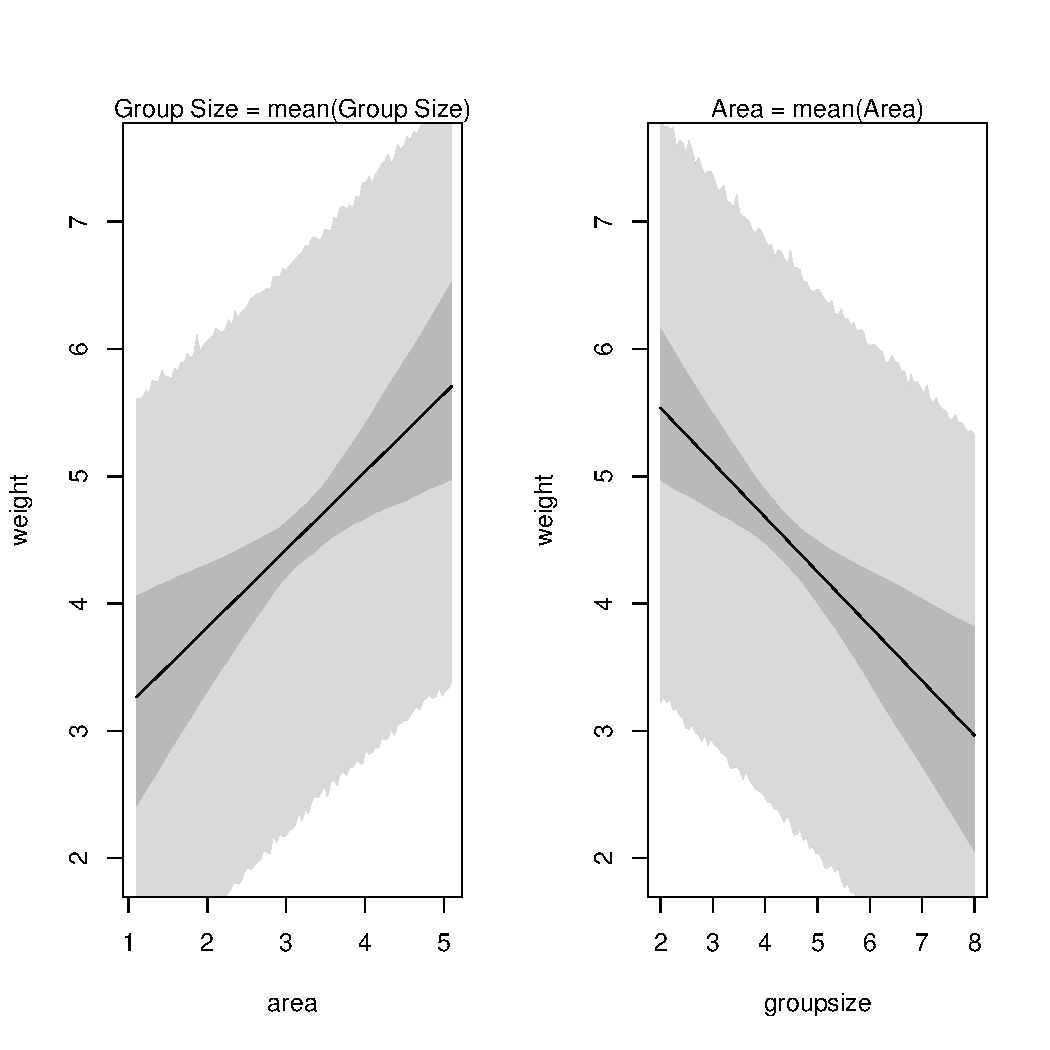
\includegraphics[width=\maxwidth]{figure/unnamed-chunk-6-1} 

\end{knitrout}

In each plot, the darker shaded region shows 95\% percentile intervals of the means, and the lighter shaded region shows 95\% prediction intervals.

When holding each variable constant at its mean, we can see that the other variable has a strong correlation with weight. In the case where area varies while group size remains constant, the correlation is strongly positive. In the opposite case, the correlation is strongly negative. The 95\% percentile intervals of the means demonstrate that a horizontal line is not included in the interval, again demonstrating that the relationship for each variable is important.

\begin{problem}{5H3}
\text{ }\\
Finally, consider the avgfood variable. Fit two more multiple regressions: (1) body weight as an additive function of avgfood and groupsize, and (2) body weight as an additive function of all three variables, avgfood and groupsize and area. Compare the results of these models to the previous models you've fit, in the first two exercises. (a) Is avgfood or area a better predictor of body weight? If you had to choose one or the other to include in a model, which would it be? Support your assessment with any tables or plots you choose. (b) When both avgfood or area are in the same model, their effects are reduced (closer to zero) and their standard errors are larger than when they are included in separate models. Can you explain this result?
\end{problem}

\begin{knitrout}
\definecolor{shadecolor}{rgb}{0.969, 0.969, 0.969}\color{fgcolor}\begin{kframe}
\begin{alltt}
\hlstd{model4} \hlkwb{<-} \hlkwd{map}\hlstd{(}
  \hlkwd{alist}\hlstd{(}
    \hlstd{weight} \hlopt{~} \hlkwd{dnorm}\hlstd{(mu, sigma),}
    \hlstd{mu} \hlkwb{<-} \hlstd{a} \hlopt{+} \hlstd{b1} \hlopt{*} \hlstd{avgfood} \hlopt{+} \hlstd{b2} \hlopt{*} \hlstd{groupsize,}
    \hlstd{a} \hlopt{~} \hlkwd{dnorm}\hlstd{(}\hlnum{10}\hlstd{,} \hlnum{10}\hlstd{),}
    \hlstd{b1} \hlopt{~} \hlkwd{dnorm}\hlstd{(}\hlnum{0}\hlstd{,} \hlnum{100}\hlstd{),}
    \hlstd{b2} \hlopt{~} \hlkwd{dnorm}\hlstd{(}\hlnum{0}\hlstd{,} \hlnum{100}\hlstd{),}
    \hlstd{sigma} \hlopt{~} \hlkwd{dunif}\hlstd{(}\hlnum{0}\hlstd{,} \hlnum{10}\hlstd{)}
  \hlstd{),} \hlkwc{data} \hlstd{= d)}

\hlkwd{precis}\hlstd{(model4)}
\end{alltt}
\begin{verbatim}
##        Mean StdDev  5.5% 94.5%
## a      4.13   0.43  3.44  4.82
## b1     3.81   1.21  1.87  5.74
## b2    -0.57   0.16 -0.82 -0.32
## sigma  1.12   0.07  1.00  1.23
\end{verbatim}
\begin{alltt}
\hlkwd{plot}\hlstd{(}\hlkwd{precis}\hlstd{(model4))}
\end{alltt}
\end{kframe}
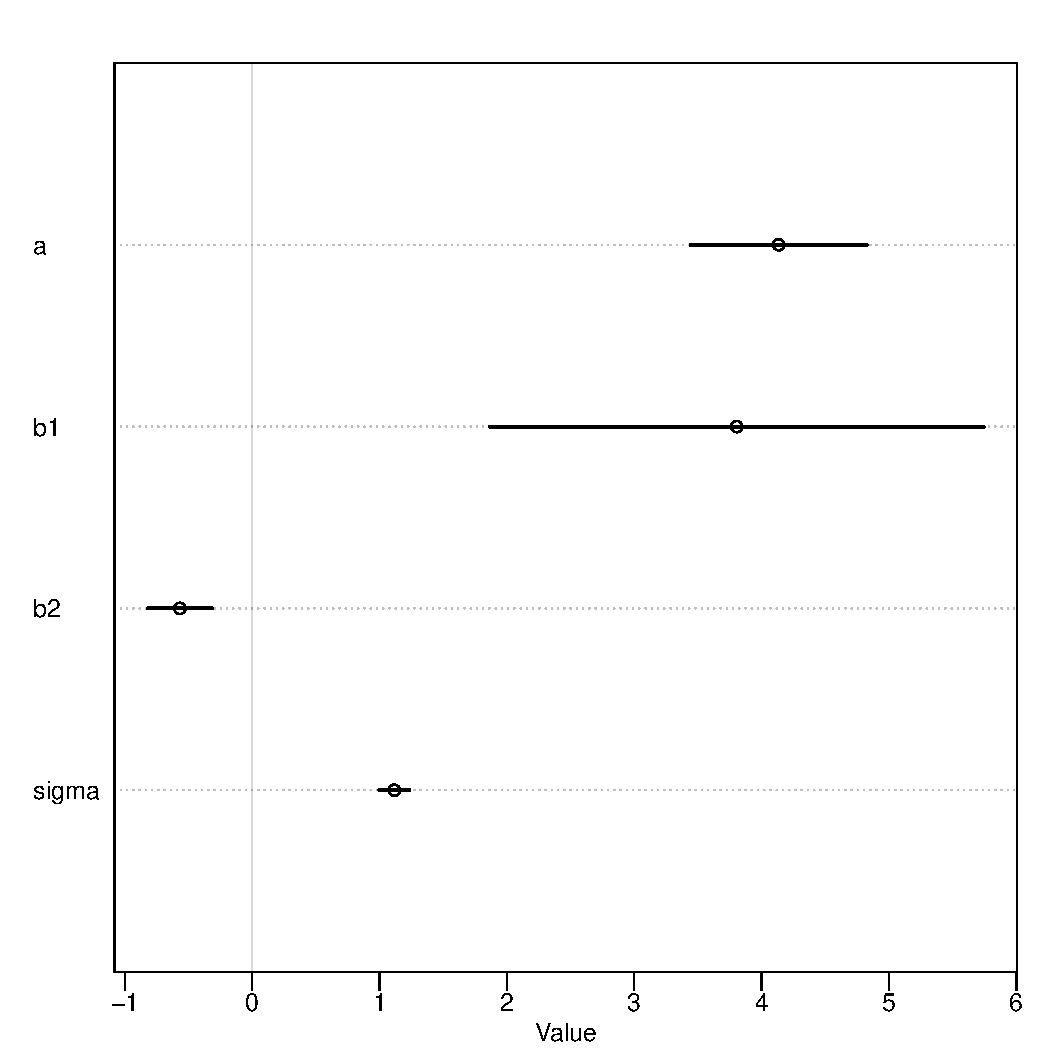
\includegraphics[width=\maxwidth]{figure/unnamed-chunk-7-1} 
\begin{kframe}\begin{alltt}
\hlstd{model5} \hlkwb{<-} \hlkwd{map}\hlstd{(}
  \hlkwd{alist}\hlstd{(}
    \hlstd{weight} \hlopt{~} \hlkwd{dnorm}\hlstd{(mu, sigma),}
     \hlstd{mu} \hlkwb{<-} \hlstd{a} \hlopt{+} \hlstd{b1} \hlopt{*} \hlstd{avgfood} \hlopt{+} \hlstd{b2} \hlopt{*} \hlstd{groupsize} \hlopt{+} \hlstd{b3} \hlopt{*} \hlstd{area,}
    \hlstd{a} \hlopt{~} \hlkwd{dnorm}\hlstd{(}\hlnum{10}\hlstd{,} \hlnum{10}\hlstd{),}
    \hlstd{b1} \hlopt{~} \hlkwd{dnorm}\hlstd{(}\hlnum{0}\hlstd{,} \hlnum{100}\hlstd{),}
    \hlstd{b2} \hlopt{~} \hlkwd{dnorm}\hlstd{(}\hlnum{0}\hlstd{,} \hlnum{100}\hlstd{),}
    \hlstd{b3} \hlopt{~} \hlkwd{dnorm}\hlstd{(}\hlnum{0}\hlstd{,} \hlnum{100}\hlstd{),}
    \hlstd{sigma} \hlopt{~} \hlkwd{dunif}\hlstd{(}\hlnum{0}\hlstd{,} \hlnum{10}\hlstd{)}
  \hlstd{),} \hlkwc{data} \hlstd{= d)}

\hlkwd{precis}\hlstd{(model5)}
\end{alltt}
\begin{verbatim}
##        Mean StdDev  5.5% 94.5%
## a      4.08   0.43  3.39  4.76
## b1     2.48   1.45  0.16  4.81
## b2    -0.61   0.16 -0.86 -0.36
## b3     0.38   0.24  0.00  0.77
## sigma  1.10   0.07  0.99  1.22
\end{verbatim}
\begin{alltt}
\hlkwd{plot}\hlstd{(}\hlkwd{precis}\hlstd{(model5))}
\end{alltt}
\end{kframe}
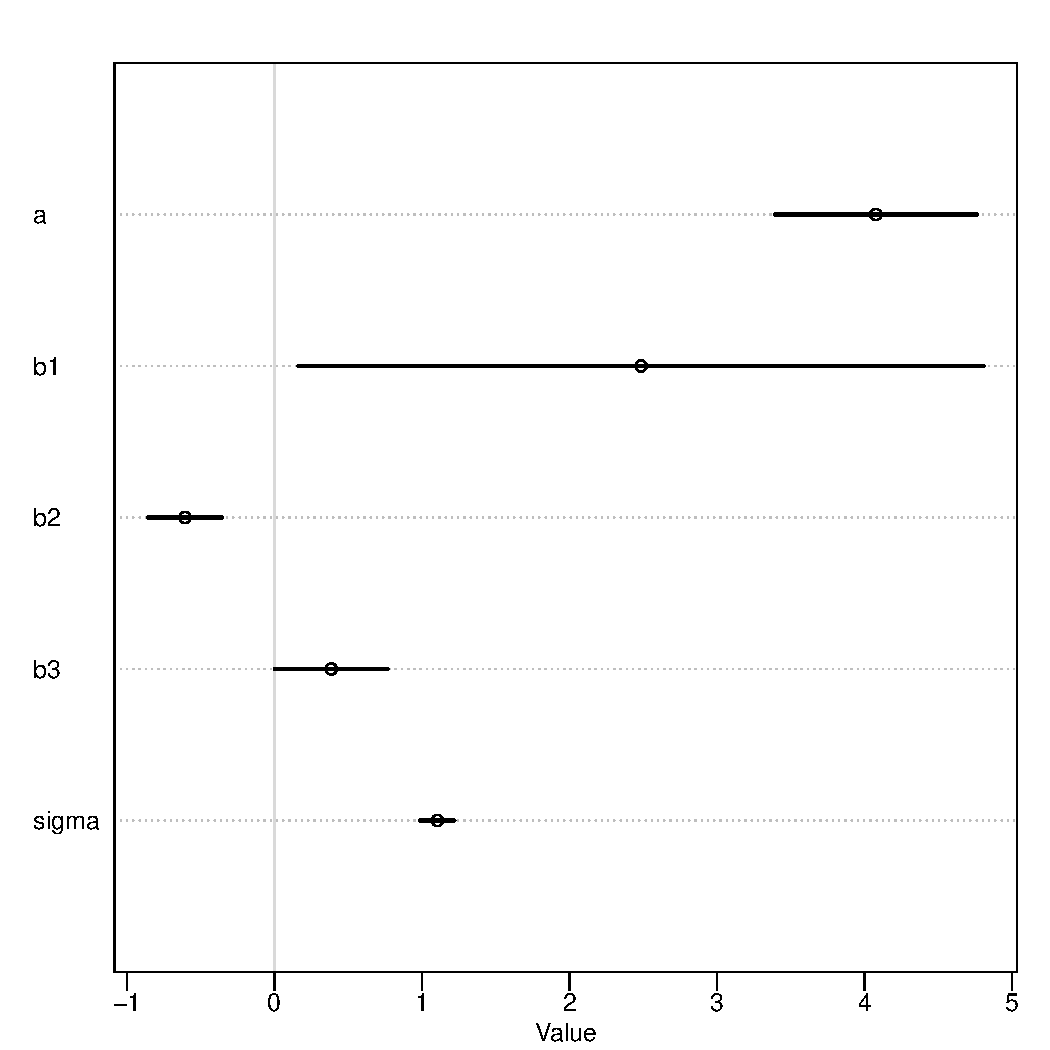
\includegraphics[width=\maxwidth]{figure/unnamed-chunk-7-2} 

\end{knitrout}

a) Let's compare avgfood and area:

\begin{knitrout}
\definecolor{shadecolor}{rgb}{0.969, 0.969, 0.969}\color{fgcolor}\begin{kframe}
\begin{alltt}
\hlstd{avgfood.seq} \hlkwb{<-} \hlkwd{seq}\hlstd{(}\hlkwc{from} \hlstd{=} \hlkwd{round}\hlstd{(}\hlkwd{min}\hlstd{(d}\hlopt{$}\hlstd{avgfood),} \hlnum{1}\hlstd{),} \hlkwc{to} \hlstd{=} \hlkwd{round}\hlstd{(}\hlkwd{max}\hlstd{(d}\hlopt{$}\hlstd{avgfood),}\hlnum{1}\hlstd{),} \hlkwc{length.out} \hlstd{=} \hlnum{100}\hlstd{)}

\hlstd{pred.data3} \hlkwb{<-}\hlkwd{data.frame}\hlstd{(}\hlkwc{avgfood} \hlstd{= avgfood.seq,} \hlkwc{groupsize} \hlstd{= G.avg)}

\hlstd{mu3} \hlkwb{<-} \hlkwd{link}\hlstd{(model4,} \hlkwc{data} \hlstd{= pred.data3)}
\end{alltt}
\begin{verbatim}
## [ 100 / 1000 ]
[ 200 / 1000 ]
[ 300 / 1000 ]
[ 400 / 1000 ]
[ 500 / 1000 ]
[ 600 / 1000 ]
[ 700 / 1000 ]
[ 800 / 1000 ]
[ 900 / 1000 ]
[ 1000 / 1000 ]

\end{verbatim}
\begin{alltt}
\hlstd{mu3.mean} \hlkwb{<-} \hlkwd{apply}\hlstd{(mu3,} \hlnum{2}\hlstd{, mean)}
\hlstd{mu3.PI} \hlkwb{<-} \hlkwd{apply}\hlstd{(mu3,} \hlnum{2}\hlstd{, PI,} \hlnum{0.95}\hlstd{)}

\hlstd{F.sim} \hlkwb{<-} \hlkwd{sim}\hlstd{(model4,} \hlkwc{data} \hlstd{= pred.data3,} \hlkwc{n} \hlstd{=} \hlnum{1e4}\hlstd{)}
\end{alltt}
\begin{verbatim}
## [ 1000 / 10000 ]
[ 2000 / 10000 ]
[ 3000 / 10000 ]
[ 4000 / 10000 ]
[ 5000 / 10000 ]
[ 6000 / 10000 ]
[ 7000 / 10000 ]
[ 8000 / 10000 ]
[ 9000 / 10000 ]
[ 10000 / 10000 ]

\end{verbatim}
\begin{alltt}
\hlstd{F.PI} \hlkwb{<-} \hlkwd{apply}\hlstd{(F.sim,} \hlnum{2}\hlstd{, PI,} \hlnum{0.95}\hlstd{)}

\hlkwd{par}\hlstd{(}\hlkwc{mfrow}\hlstd{=}\hlkwd{c}\hlstd{(}\hlnum{1}\hlstd{,}\hlnum{2}\hlstd{))}

\hlkwd{plot}\hlstd{(weight} \hlopt{~} \hlstd{area,} \hlkwc{data} \hlstd{= d,} \hlkwc{type} \hlstd{=} \hlstr{"n"}\hlstd{)}
\hlkwd{mtext}\hlstd{(}\hlstr{"Area w/ Group Size = mean(Group Size)"}\hlstd{)}
\hlkwd{lines}\hlstd{(area.seq, mu1.mean)}
\hlkwd{shade}\hlstd{(mu1.PI, area.seq)}
\hlkwd{shade}\hlstd{(A.PI, area.seq)}

\hlkwd{plot}\hlstd{(weight} \hlopt{~} \hlstd{avgfood,} \hlkwc{data} \hlstd{= d,} \hlkwc{type} \hlstd{=} \hlstr{"n"}\hlstd{)}
\hlkwd{mtext}\hlstd{(}\hlstr{"Avgfood w/ Group Size = mean(Group Size)"}\hlstd{)}
\hlkwd{lines}\hlstd{(avgfood.seq, mu3.mean)}
\hlkwd{shade}\hlstd{(mu3.PI, avgfood.seq)}
\hlkwd{shade}\hlstd{(F.PI, avgfood.seq)}
\end{alltt}
\end{kframe}
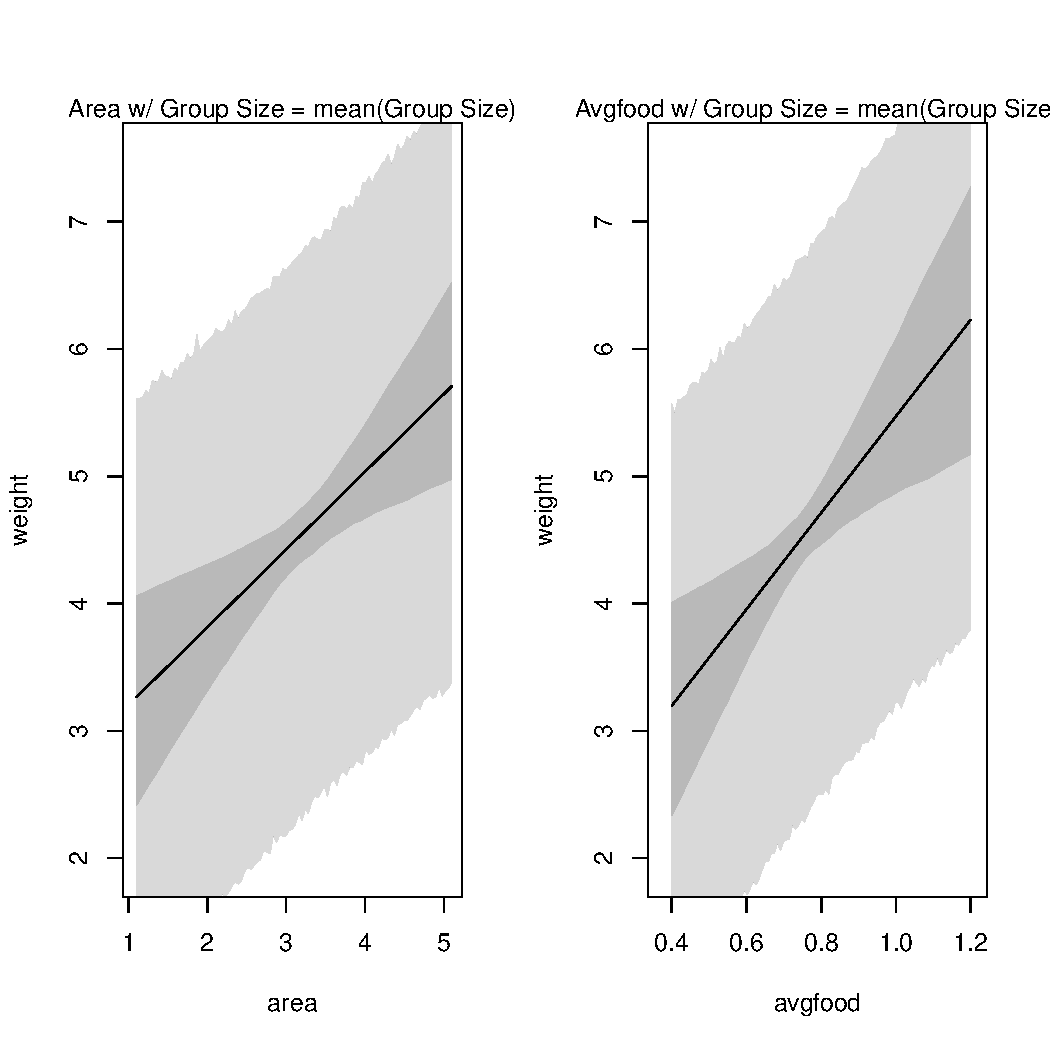
\includegraphics[width=\maxwidth]{figure/unnamed-chunk-8-1} 

\end{knitrout}

Holding group size constant at its mean, it appears that avgfood has a slightly more positive correlation with weight than area does. As a result, we should use avgfood in place of area.

b) This occurs due to the presence of multicollinearity in our predictors, which we will demonstrate below:

\begin{knitrout}
\definecolor{shadecolor}{rgb}{0.969, 0.969, 0.969}\color{fgcolor}\begin{kframe}
\begin{alltt}
\hlkwd{print}\hlstd{(}\hlkwd{cor}\hlstd{(d}\hlopt{$}\hlstd{avgfood, d}\hlopt{$}\hlstd{area))}
\end{alltt}
\begin{verbatim}
## [1] 0.8831038
\end{verbatim}
\end{kframe}
\end{knitrout}

We can see that the variables avgfood and area are highly positively correlated. Now to show that the posterior distributions for their coefficients are highly correlated as well:

\begin{knitrout}
\definecolor{shadecolor}{rgb}{0.969, 0.969, 0.969}\color{fgcolor}\begin{kframe}
\begin{alltt}
\hlstd{post} \hlkwb{<-} \hlkwd{extract.samples}\hlstd{(model5)}
\hlkwd{names}\hlstd{(post)} \hlkwb{<-} \hlkwd{c}\hlstd{(}\hlstr{"intercept"}\hlstd{,} \hlstr{"avgfood_coeff"}\hlstd{,} \hlstr{"groupsize coeff"}\hlstd{,} \hlstr{"area_coeff"}\hlstd{,} \hlstr{"sigma"}\hlstd{)}
\hlkwd{plot}\hlstd{(avgfood_coeff} \hlopt{~} \hlstd{area_coeff, post,} \hlkwc{col}\hlstd{=}\hlkwd{col.alpha}\hlstd{(rangi2,} \hlnum{0.1}\hlstd{),} \hlkwc{pch} \hlstd{=} \hlnum{16}\hlstd{)}
\end{alltt}
\end{kframe}
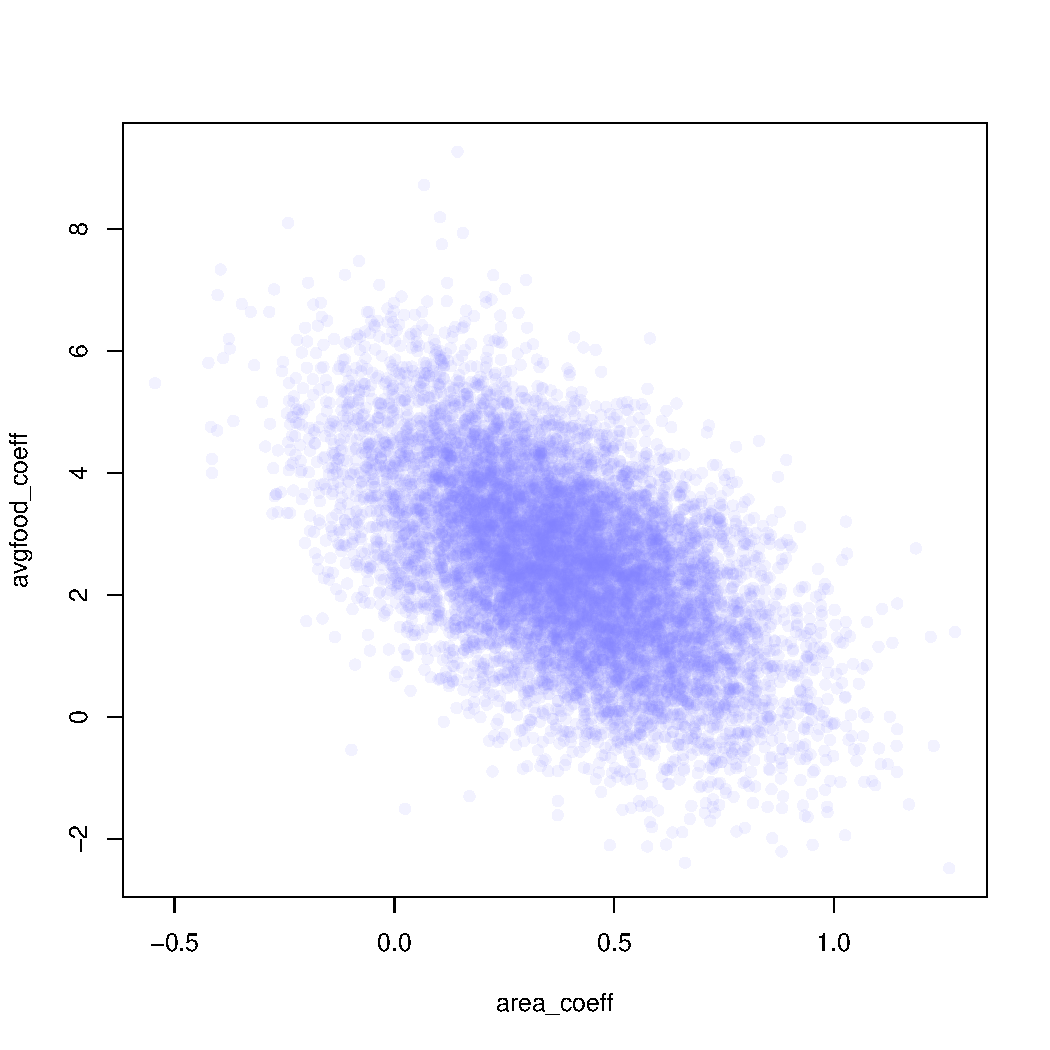
\includegraphics[width=\maxwidth]{figure/unnamed-chunk-10-1} 

\end{knitrout}

We can see that the two coefficients are highly negatively correlated. From the correlation of the variables and coefficients, we can see that both variables contain nearly the same information. Thus, only one should be included in the model.

\end{document}
